% STATUS: SUPPORT -- AR(1)-first independent companion to 4state_del_hd.tex
% ======================================================
% Compile: xelatex 4state_del_hd_ar1.tex
% Path:    reference/eq17_analysis/derivation/4state_del_hd_ar1.tex
% AR(1)-first standalone derivation of the 4-state eq17 controller + closed-loop EKF.
% Independent companion to 4state_del_hd.tex: identical main line (equation of motion
% -> implementable control effort), but from the Parameter model onward the gain state
% is presented directly as the corrected AR(1) reverting model (F_e(4,4)=lc, predict
% reverts to a_x_det, Q44 = AR(1) white-driver variance) -- no random-walk-then-correct
% two-pass. Per-axis state x = [delta_x_1, delta_x_2, delta_x_3, a_x].
% Style mirrors 4state_del_hd (monochrome, \fbox on key results, terse, math only).
% ======================================================
% fontset=none: this derivation has no CJK text, so do not load Chinese fonts
% (this Windows box lacks KaiTi/FangSong); output is identical, compiles anywhere.
\documentclass[11pt,a4paper,fontset=none]{ctexart}

\usepackage[fleqn]{amsmath}
\usepackage{amssymb,bm}
\usepackage{empheq}
\setlength{\mathindent}{0pt}
\usepackage{geometry}
\geometry{margin=2.0cm}
\usepackage{enumitem}
\usepackage{array,booktabs}
\usepackage{titlesec}
\usepackage{graphicx}

\setlength{\parindent}{0pt}
\setlength{\parskip}{0.3em}
\setlength{\abovedisplayskip}{4pt}
\setlength{\belowdisplayskip}{4pt}
\setlength{\abovedisplayshortskip}{2pt}
\setlength{\belowdisplayshortskip}{2pt}

\newcommand{\lc}{\lambda_c}
\newcommand{\hd}[1]{\par\medskip\noindent\underline{\textbf{#1}}\par\nobreak\vspace{0.2ex}}

\begin{document}

\hd{Equation of motion}
\[ x[k+1] = x[k] + a_x[k]\{f_{dx}[k] + f_T[k]\} + \delta x_D[k], \]

\hd{Motion error}
\[ \delta x[k+1] = \delta x[k] + \Delta x_d[k] - a_x[k]\{f_{dx}[k] + f_T[k]\} - \delta x_D[k], \]

$\delta x[k] = x_d[k] - x[k]$, $x_d[k]$ is the desired motion trajectory, $\delta x_D[k]$ is the motion error caused by the disturbance, and $\Delta x_d[k] = x_d[k+1] - x_d[k]$ is the desired motion step size.

\hd{Measurement} (\textit{d}-step delay)
\[ \delta x_m[k] = \delta x[k-d] + n_x[k], \]

\noindent\underline{\textbf{Control objective}}: $\;\delta x[k+1] = \lc \cdot \delta x[k];\quad 0 \le \lc < 1$

\medskip
\textit{Ideal control effort (no measurement delay)}:
\[ \bar f_{dx}[k] = a_x^{-1}[k]\{\Delta x_d[k] + (1-\lc)\,\bm{\delta x[k]} - \delta x_D[k]\} \]

\textit{Motion error}:
\[ \delta x[k+1] = \delta x[k] + \Delta x_d[k] - a_x[k]\{\bar f_{dx}[k] + f_T[k]\} - \delta x_D[k] = \lc \cdot \delta x[k] - a_x[k] f_T[k] \]

\textit{d-step measurement delay}:
\[ \bm{\delta x[k]} = \delta x[k-d] + \sum_{i=1}^{d}\Delta x_d[k-i] - \sum_{i=1}^{d} a_x[k-i]\{f_{dx}[k-i] + f_T[k-i]\} - \sum_{i=1}^{d}\delta x_D[k-i] \]

\textit{Ideal control effort (with d-step measurement delay)}:
\[
\begin{aligned}
\bar{\bar f}_{dx}[k] = a_x^{-1}[k]\Big\{
& \underbrace{\Big[\Delta x_d[k] + (1-\lc)\textstyle\sum_{i=1}^{d}\Delta x_d[k-i]\Big]}_{\Delta x_d^{d}[k]}
+ (1-\lc)\Big[\delta x[k-d] - \textstyle\sum_{i=1}^{d} a_x[k-i] f_{dx}[k-i]\Big] \\
& - \underbrace{\Big[\delta x_D[k] + (1-\lc)\textstyle\sum_{i=1}^{d}\delta x_D[k-i]\Big]}_{\delta x_D^{d}[k]}
\Big\}
\end{aligned}
\]

\textit{Motion error}:
\[
\delta x[k+1] = \lc \cdot \delta x[k] - \underbrace{\Big\{ a_x[k] f_T[k] + (1-\lc)\textstyle\sum_{i=1}^{d} a_x[k-i] f_T[k-i] \Big\}}_{\delta x_T^{d}[k]}
\]

\hd{Implementable control effort}
\begin{empheq}[box=\fbox]{equation*}
f_{dx}[k] = \hat a_x^{-1}[k]\Big\{ \Delta x_d^{d}[k] + (1-\lc)\Big[\delta x_m[k] - \textstyle\sum_{i=1}^{d}\hat a_x[k-i] f_{dx}[k-i]\Big] \Big\}
\end{empheq}

\hd{Motion error}
\[ \delta x[k+1] = \lc \cdot \delta x[k] - a_x[k]\big[ f_{dx}[k] - \bar{\bar f}_{dx}[k] \big] - \delta x_T^{d}[k] \]

\[ a_x[k]\,\bar{\bar f}_{dx}[k] = \Delta x_d^{d}[k] + (1-\lc)\Big[\delta x[k-d] - \textstyle\sum_{i=1}^{d} a_x[k-i] f_{dx}[k-i]\Big] - \delta x_D^{d}[k] \]

\[
a_x[k]\, f_{dx}[k] = \big(1 + e_{a_x}[k]\,\hat a_x^{-1}[k]\big)\Big\{ \Delta x_d^{d}[k]
+ (1-\lc)\Big[\big(\delta x[k-d] + n_x[k]\big) - \textstyle\sum_{i=1}^{d}\hat a_x[k-i] f_{dx}[k-i]\Big] \Big\}
\]

\[
\begin{aligned}
a_x[k]\, f_{dx}[k] - a_x[k]\,\bar{\bar f}_{dx}[k] ={}& e_{a_x}[k]\, f_{dx}[k] + (1-\lc) n_x[k] \\
&+ (1-\lc)\textstyle\sum_{i=1}^{d}\big(a_x[k-i] - \hat a_x[k-i]\big) f_{dx}[k-i] + \delta x_D^{d}[k]
\end{aligned}
\]

\hd{Parameter model}
\[ a_x[k] = a_{x_{det}}[k] + a_{x_{ram}}[k]; \qquad a_{x_{ram}}[k] \approx a'_x[k]\, x_{ram}[k] \]
\[
\begin{aligned}
a_x[k+1] &= a_{x_{det}}[k+1] + a_{x_{ram}}[k+1]
= \underbrace{\big\{ a_{x_{det}}[k] + a_{x_{ram}}[k] \big\}}_{a_x[k]} + \Delta a_x[k]
+ \underbrace{\big\{ a_{x_{ram}}[k+1] - a_{x_{ram}}[k] \big\}}_{\Delta a_{ram}[k]} \\
&= a_x[k] + \Delta a_x[k] + \Delta a_{ram}[k]
\end{aligned}
\]
\[
\Delta a_x[k] = a_{x_{det}}[k+1] - a_{x_{det}}[k] = a'_x[k]\,\Delta h_d[k]\ (\text{from } p_d),
\qquad
\Delta a_{ram}[k] = a'_x[k]\,\Delta x_{ram}[k]
\]
$\Delta h_d[k] = h_d[k+1] - h_d[k]$ (desired-trajectory height increment).

\hd{Gain dynamics --- $a_{x_{ram}}$ is first-order autoregressive (AR(1))}
\textbf{Assumption} ($x = x_{det}+x_{ram}$, perfect tracking $x_{det}=x_d$): $\;\delta x = x_d - x = -x_{ram}$ (zero-mean), $\;x_{ram} = -\delta x$; ideal closed loop ($\hat a_x = a_x$, $\delta x_D^{d}\!\equiv\!0$) gives $\delta x[k+1] = \lc\,\delta x[k] - \varepsilon[k]$ ($\varepsilon$: closed-loop residual, defined in the boxed motion error below).
\[ a_{x_{ram}}[k+1] = -a'_x\,\delta x[k+1] = -a'_x\big(\lc\,\delta x[k]-\varepsilon[k]\big) = \lc\, a_{x_{ram}}[k] + a'_x\,\varepsilon[k] \]
\[
\begin{aligned}
a_x[k+1] &= \big(a_{x_{det}}[k]+\Delta a_x[k]\big) + \big(\lc\,a_{x_{ram}}[k]+a'_x\,\varepsilon[k]\big) \\
&= \big(a_{x_{det}}[k]+\Delta a_x[k]\big) + \lc\big(a_x[k]-a_{x_{det}}[k]\big) + a'_x\,\varepsilon[k] \\
&= \underbrace{\lc\, a_x[k]}_{\mathbf F_e(4,4)=\lc} + \underbrace{(1-\lc)\,a_{x_{det}}[k] + \Delta a_x[k]}_{\text{known input}} + \underbrace{a'_x\,\varepsilon[k]}_{q_4[k]}
\end{aligned}
\]
\begin{empheq}[box=\fbox]{equation*}
\mathbf F_e(4,4) = \lc
\end{empheq}

\textit{Parameter estimator} (predict reverts to $a_{x_{det}}$): \quad $\hat a_x[k+1] = \lc\,\hat a_x[k] + (1-\lc)\,a_{x_{det}}[k] + \Delta a_x[k]$

\textit{Parameter estimation error}: \quad $e_{a_x}[k] = a_x[k] - \hat a_x[k]$

\textit{Estimation error dynamics}: \quad $e_{a_x}[k+1] = \lc\, e_{a_x}[k] + a'_x\,\varepsilon[k]$

\newpage
\[
a_x[k-i] - \hat a_x[k-i] = e_{a_x}[k-i]
\;\overset{(\dagger)}{\approx}\; e_{a_x}[k] - \sum_{j=1}^{i}\Delta a_{ram}[k-j]
\]
{\small $(\dagger)$ feedforward form $e_{a_x}[k{+}1]{=}e_{a_x}[k]{+}\Delta a_{ram}$ is exact; the AR(1) predictor gives $e_{a_x}[k{+}1]{=}\lc e_{a_x}{+}a'_x\varepsilon$, altering the expansion by $O\big((1{-}\lc)e_{a_x}\big)$ which enters only $\delta x_{\delta af}^{d}\ (\ll \delta x_T^{d}$ in $\varepsilon)$.}

\[
\begin{aligned}
a_x[k]\, f_{dx}[k] - a_x[k]\,\bar{\bar f}_{dx}[k] \approx{}&
e_{a_x}[k]\,\underbrace{\Big\{ f_{dx}[k] + (1-\lc)\textstyle\sum_{i=1}^{d} f_{dx}[k-i] \Big\}}_{F_{dx}[k]} \\
&- \underbrace{\Big\{ (1-\lc)\textstyle\sum_{i=1}^{d} (d+1-i)\, f_{dx}[k-i]\,\Delta a_{ram}[k-i] \Big\}}_{\delta x_{\delta af}^{d}[k]} \\
&+ \delta x_D^{d}[k] + (1-\lc) n_x[k]
\end{aligned}
\]

\begin{empheq}[box=\fbox]{equation*}
\delta x[k+1] = \lc \cdot \delta x[k] - F_{dx}[k]\cdot e_{a_x}[k] - \delta x_D^{d}[k]
- \underbrace{\Big\{ \delta x_T^{d}[k] - \delta x_{\delta af}^{d}[k] + (1-\lc) n_x[k] \Big\}}_{\varepsilon[k]}
\end{empheq}

\hd{State equation} \;{\small ($\delta x_D^{d}\!\equiv\!0$: disturbance not modelled)}
\[
\begin{aligned}
\delta x_1[k+1] &= \delta x_2[k] \\
\delta x_2[k+1] &= \delta x_3[k] \\
\delta x_3[k+1] &= \lc \cdot \delta x_3[k] - F_{dx}[k]\cdot e_{a_x}[k] - \varepsilon[k] \\
a_x[k+1] &= \lc\, a_x[k] + (1-\lc)\,a_{x_{det}}[k] + \Delta a_x[k] + a'_x\,\varepsilon[k]
\end{aligned}
\]

\hd{Output equation}
\[
\begin{cases}
y_1[k] = \delta x_m[k] = \delta x_1[k] + \underbrace{n_x[k]}_{r_1[k]} \\[1.8ex]
y_2[k] = \underbrace{a_x[k-d] + n_a[k]}_{a_{xm}[k]} = a_x[k] - \textstyle\sum_{i=1}^{d}\Delta a_x[k-i] + \underbrace{\Big\{ n_a[k] - \textstyle\sum_{i=1}^{d}\Delta a_{ram}[k-i] \Big\}}_{r_2[k]}
\end{cases}
\]
\[
\mathbf{H} = \begin{bmatrix} 1 & 0 & 0 & 0 \\ 0 & 0 & 0 & 1 \end{bmatrix},
\qquad
\mathbf{c}[k] = \begin{bmatrix} 0 \\ \textstyle\sum_{i=1}^{d}\Delta a_x[k-i] \end{bmatrix}\ (\text{known}),
\qquad
\mathbf{y}[k] = \mathbf{H}\mathbf{x}[k] - \mathbf{c}[k] + \mathbf{r}[k]
\]

\newpage
\hd{Past-error expansion under AR(1) $(\dagger)$}
\textit{Two predictors, two $e_{a_x}$ recursions} (predict-only):
\[
\begin{aligned}
\text{feedforward:}\quad & e_{a_x}[k+1] = e_{a_x}[k] + \Delta a_{ram}[k]
   \ \Rightarrow\ e_{a_x}[k-i] = e_{a_x}[k] - \textstyle\sum_{j=1}^{i}\Delta a_{ram}[k-j] \quad(\text{exact}) \\
\text{AR(1):}\quad & e_{a_x}[k+1] = \lc\, e_{a_x}[k] + a'_x\varepsilon[k]
   \ \Rightarrow\ e_{a_x}[k-i] = \lc^{-i}\big(e_{a_x}[k] - \textstyle\sum_{j=1}^{i}\lc^{j-1}a'_x\varepsilon[k-j]\big)
\end{aligned}
\]
\textit{Difference} ($\Delta_i := e_{a_x}^{\mathrm{AR(1)}}[k-i] - e_{a_x}^{\mathrm{ff}}[k-i]$):
\[ \Delta_i = \underbrace{(\lc^{-i}-1)\,e_{a_x}[k]}_{\text{reverting}}
   - \lc^{-i}\sum_{j=1}^{i}\lc^{j-1}a'_x\varepsilon[k-j]
   + \sum_{j=1}^{i}\Delta a_{ram}[k-j] \]
\textit{Leading order} (small $i$, $\lc^{-i} \approx 1 + i(1-\lc)$):
\[ (\lc^{-i}-1)\,e_{a_x}[k] \approx i(1-\lc)\,e_{a_x}[k] = O\big((1-\lc)\,e_{a_x}\big) \]
$\Rightarrow$ the feedforward expansion errs by $O((1-\lc)e_{a_x})$, entering $\varepsilon$ only through $\delta x_{\delta af}^{d}\ (\ll \delta x_T^{d})$; numerically $Q_{33}/R_{22}$ with $\mathrm{Var}(\Delta a_{ram})$ vs $q_4$ leaves $\hat a_x$ unchanged.

\newpage
\hd{Closed-loop Estimator}
\[ e_{\delta x_1}[k] = \delta x_1[k] - \delta \hat x_1[k] \]
\[ e_{a_x}[k] = a_x[k] - \hat a_x[k] \]
\[ e_{y_1}[k] = y_1[k] - \hat y_1[k] = \delta x_m[k] - \delta \hat x_1[k] = e_{\delta x_1}[k] + \underbrace{n_x[k]}_{r_1[k]} \]
\[
\begin{aligned}
e_{y_2}[k] &= y_2[k] - \hat y_2[k] = a_{xm}[k] - \Big(\hat a_x[k] - \textstyle\sum_{i=1}^{d}\Delta a_x[k-i]\Big) \\
&= \Big(a_x[k] - \textstyle\sum_{i=1}^{d}\Delta a_x[k-i] + r_2[k]\Big) - \hat a_x[k] + \textstyle\sum_{i=1}^{d}\Delta a_x[k-i] \\
&= e_{a_x}[k] + \underbrace{\Big\{ n_a[k] - \textstyle\sum_{i=1}^{d}\Delta a_{ram}[k-i] \Big\}}_{r_2[k]}
\end{aligned}
\]
\[
\begin{aligned}
\delta \hat x_1[k+1] &= \delta \hat x_2[k] + \ell_{11}[k]\, e_{y_1}[k] + \ell_{12}[k]\, e_{y_2}[k] \\
\delta \hat x_2[k+1] &= \delta \hat x_3[k] + \ell_{21}[k]\, e_{y_1}[k] + \ell_{22}[k]\, e_{y_2}[k] \\
\delta \hat x_3[k+1] &= \lc \cdot \delta \hat x_3[k] + \ell_{31}[k]\, e_{y_1}[k] + \ell_{32}[k]\, e_{y_2}[k] \\
\hat a_x[k+1] &= \lc\,\hat a_x[k] + (1-\lc)\,a_{x_{det}}[k] + \Delta a_x[k] + \ell_{41}[k]\, e_{y_1}[k] + \ell_{42}[k]\, e_{y_2}[k]
\end{aligned}
\]

\hd{Error dynamics}
\[
\begin{aligned}
e_{\delta x_1}[k+1] &= e_{\delta x_2}[k] - \ell_{11}[k]\, e_{\delta x_1}[k] - \ell_{12}[k]\, e_{a_x}[k] \\
e_{\delta x_2}[k+1] &= e_{\delta x_3}[k] - \ell_{21}[k]\, e_{\delta x_1}[k] - \ell_{22}[k]\, e_{a_x}[k] \\
e_{\delta x_3}[k+1] &= \lc \cdot e_{\delta x_3}[k] - F_{dx}[k]\cdot e_{a_x}[k] - \ell_{31}[k]\, e_{\delta x_1}[k] - \ell_{32}[k]\, e_{a_x}[k] - \underbrace{\varepsilon[k]}_{q_3[k]} \\
e_{a_x}[k+1] &= \lc\, e_{a_x}[k] - \ell_{41}[k]\, e_{\delta x_1}[k] - \ell_{42}[k]\, e_{a_x}[k] + \underbrace{a'_x\,\varepsilon[k]}_{q_4[k]}
\end{aligned}
\]

\newpage
\begin{empheq}[box=\fbox]{equation*}
\mathbf{F}_e[k] =
\begin{bmatrix}
0 & 1 & 0 & 0 \\
0 & 0 & 1 & 0 \\
0 & 0 & \lc & -F_{dx}[k] \\
0 & 0 & 0 & \lc
\end{bmatrix}
\end{empheq}

\[ F_{dx}[k] = f_{dx}[k] + (1-\lc)\sum_{i=1}^{d} f_{dx}[k-i] \]

\[ \mathbf{e}[k+1] = \mathbf{F}_e[k]\,\mathbf{e}[k] - \mathbf{L}[k]\,\mathbf{H}\,\mathbf{e}[k] + \mathbf{q}[k] - \mathbf{L}[k]\,\mathbf{r}[k] \]

\newpage
\hd{Process / measurement noise variances}
\textbf{Assumption} ($x = x_{det}+x_{ram}$, perfect tracking): $\;x_{ram} = -\delta x$ (zero-mean), $\;a'_x := \dfrac{d a_x}{d h} = -\dfrac{a_x K_h}{R}$, $\;K_h = \dfrac{1}{c}\dfrac{dc}{d\bar h}$ (wall sensitivity).

\textbf{Closed-loop tracking variance} (thermal-driven, $\hat a_x = a_x$):
\[ \mathrm{Var}(x_{ram}) = \mathrm{Var}(\delta x) = C_{\delta x}\,\sigma^2_{\delta h}, \qquad C_{\delta x} = 2 + \frac{1}{1-\lc^2}, \qquad \sigma^2_{\delta h} := 4 k_B T\, a_x \]

\textbf{(i) True increment} $\Delta a_{ram} = a'_x\,\Delta x_{ram}$ \;($\rho_1 = \mathrm{Cov}(x_{ram}[k{+}1],x_{ram}[k])/\mathrm{Var}(x_{ram})$, lag-1 autocorr):
\[ \mathrm{Var}(\Delta x_{ram}) = 2(1-\rho_1)\,\mathrm{Var}(x_{ram}), \qquad
   \rho_1 = \lc + \frac{2(1-\lc)}{C_{\delta x}} \;\Rightarrow\; 1-\rho_1 = \frac{1}{(1+\lc)\,C_{\delta x}} \]
\begin{empheq}[box=\fbox]{equation*}
\mathrm{Var}(\Delta a_{ram}) = a'^2_x\cdot \underbrace{2(1-\rho_1)\,C_{\delta x}}_{=\,2/(1+\lc)}\,\sigma^2_{\delta h}
= \frac{2}{1+\lc}\,a'^2_x\,\sigma^2_{\delta h}
\qquad (\to Q_{33}^{\mathrm{randgain}},\ R_{22}^{\mathrm{delay}})
\end{empheq}

\textbf{(ii) AR(1) white driver} $w_4 = a'_x\,\varepsilon$ \;($\mathrm{Var}(\varepsilon) = (1-\lc^2)\,\mathrm{Var}(\delta x)$ since $\delta x$ is AR(1)):
\begin{empheq}[box=\fbox]{equation*}
q_4 = a'^2_x\,\mathrm{Var}(\varepsilon) = (1-\lc^2)\,C_{\delta x}\,a'^2_x\,\sigma^2_{\delta h} = (3-2\lc^2)\,a'^2_x\,\sigma^2_{\delta h}
\qquad (\to Q_{44})
\end{empheq}

\textbf{Self-consistency} (AR(1) steady-state variance $=$ true gain variance):
\[ \frac{q_4}{1-\lc^2} = C_{\delta x}\,a'^2_x\,\sigma^2_{\delta h} = \mathrm{Var}(a_{x_{ram}}) \;\checkmark \]

\textbf{Impl.}: $K_h,\ \sigma^2_{\delta h}=4k_BT\,a_\perp$ evaluated at $\bar h_{\mathrm{meas}}$ ($p_m$); gain $a_x\to\hat a_x$ (estimate); reversion target $a_{x_{det}}$ from $p_d$.

\newpage
\hd{Original random-walk $Q_{44}$ --- the mismatch}
\textbf{Original model} (RW, $\mathbf F_e(4,4)=1$): predict mean and $Q_{44}$ are mutually consistent,
\[ \hat a_x[k+1] = \hat a_x[k] + \Delta a_x[k], \qquad Q_{44} = \mathrm{Var}(\Delta a_{ram}). \]

\textbf{True increment} (from $a_{x_{ram}}[k+1]=\lc\,a_{x_{ram}}[k]+a'_x\varepsilon[k]$):
\[ \Delta a_{ram}[k] = a_{x_{ram}}[k+1]-a_{x_{ram}}[k]
   = \underbrace{(\lc-1)\,a_{x_{ram}}[k]}_{\text{reversion (spring)}}
   + \underbrace{a'_x\,\varepsilon[k]}_{\text{white}} \]

\textbf{Mismatch}: RW puts the \emph{whole} $\Delta a_{ram}$ into $Q_{44}$ --- it treats the deterministic reversion $(\lc-1)a_{x_{ram}}$ as white noise; $\mathbf F_e(4,4)=1$ keeps no spring, so the modelled gain variance is unbounded while the true gain is bounded:
\[ \text{RW: } P_a[k+1]=P_a[k]+Q_{44}\ \nearrow\infty
   \qquad
   \text{AR(1): } P_a[k+1]=\lc^2 P_a[k]+q_4 \to \tfrac{q_4}{1-\lc^2} \]

\textbf{Fix}: move the reversion into the dynamics ($\mathbf F_e(4,4)=\lc$, predict reverts to $a_{x_{det}}$), keep only the white driver in $Q_{44}$:
\[ \underbrace{\mathrm{Var}(\Delta a_{ram}) = \tfrac{2}{1+\lc}\,a'^2_x\sigma^2_{\delta h}}_{\text{RW }Q_{44}}
   \;\longrightarrow\;
   \underbrace{q_4 = (3-2\lc^2)\,a'^2_x\sigma^2_{\delta h}}_{\text{AR(1) }Q_{44}} \]

\textbf{Effect} (1\,Hz, near wall, $z$-axis): $\;P_a/\mathrm{Var}(a_{x_{ram}}):\ 19.67 \to 0.78,\quad |\hat a_z - a_z|:\ 9.4\% \to 0.4\%$.

\newpage
\hd{Single-seed time series (1\,Hz, near wall, $z$-axis)}

\medskip
\noindent\begin{minipage}{\linewidth}\centering
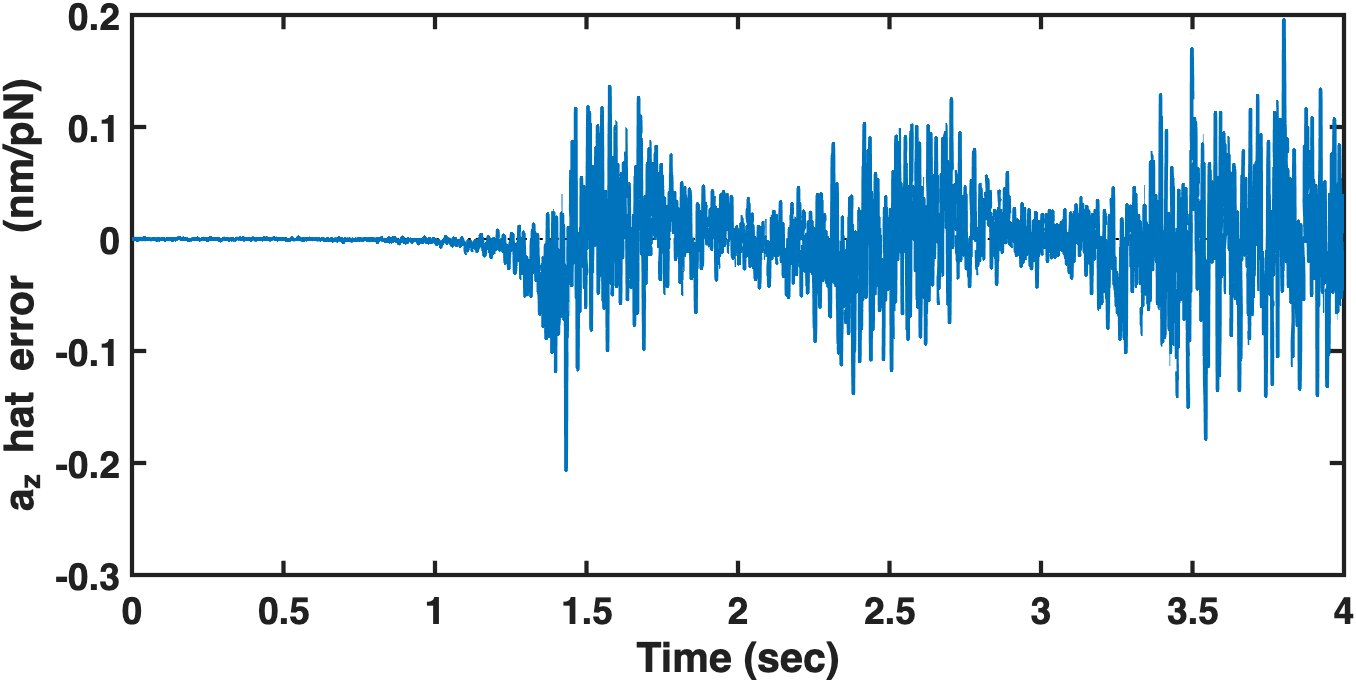
\includegraphics[width=0.9\textwidth]{figures/fig_ar1_az_err_z_1hz.png}\\[0.4ex]
{\small\itshape $a_z$ estimation error $\hat a_z - a_z$.}
\end{minipage}

\medskip
\noindent\begin{minipage}{\linewidth}\centering
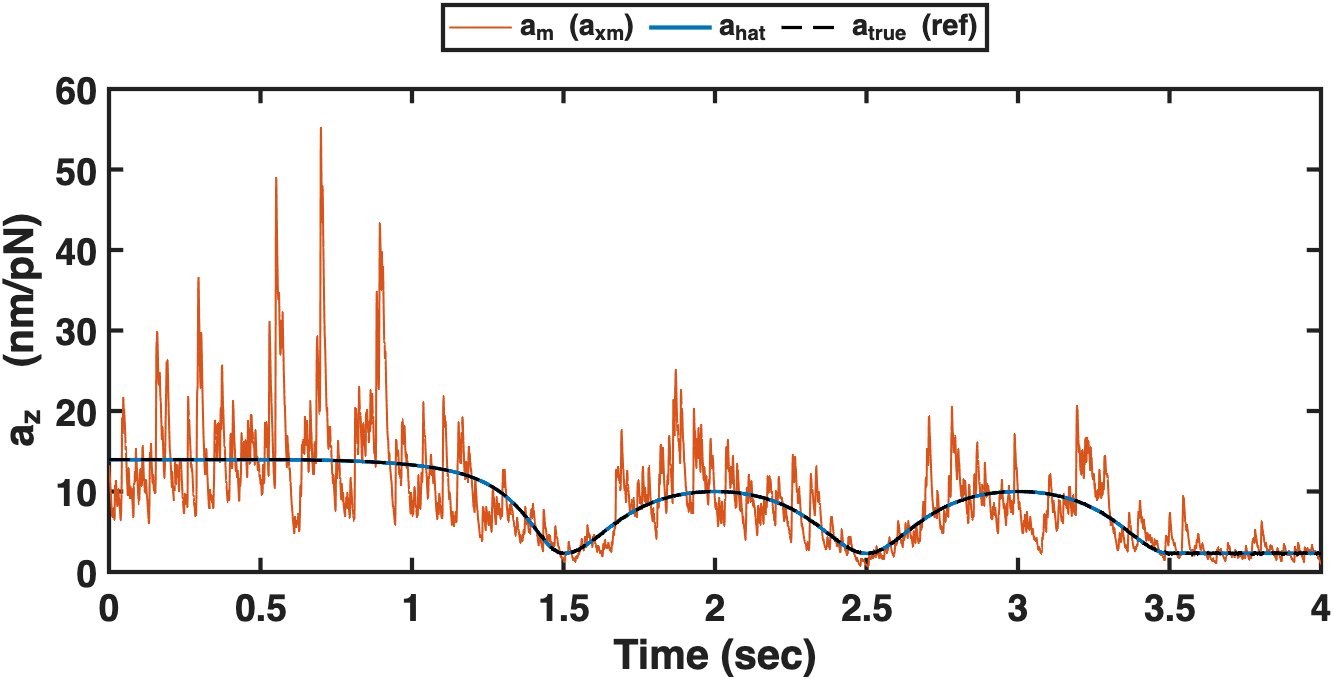
\includegraphics[width=0.9\textwidth]{figures/fig_ar1_am_vs_ahat_z_1hz.png}\\[0.4ex]
{\small\itshape $a_z$: measurement $a_m$, EKF estimate $\hat a_x$, truth $a_{true}$.}
\end{minipage}

\newpage
\hd{Decoupling from the known wall model --- $a_{x_{det}}$, $a'_x$ from model-free sources}
Both $a_{x_{det}}[k]$ (reversion target) and $a'_x[k]$ (feedforward slope, via $\Delta a_x[k]=a'_x[k]\Delta h_d[k]$) above are read from the \emph{known} wall model $c(\bar h)$. For an unknown wall, replace them with model-free, exogenous quantities --- the state stays 4-dimensional, no augmented slope/level state is added:
\[
\hat a_{x_{det}}[k+1] = (1-\alpha)\,\hat a_{x_{det}}[k] + \alpha\,a_{xm}[k+1]
\qquad(\text{EWMA of }a_{xm}\text{; needs only }\lc,\,4k_BT,\text{ not }c(\bar h))
\]
\begin{empheq}[box=\fbox]{equation*}
\hat a'_x[k] =
\begin{cases}
(1-\beta)\,\hat a'_x[k-1] \;+\; \beta\,\dfrac{\hat a_x[k]-\hat a_x[k-1]}{\Delta h_d[k-1]}, & |\Delta h_d[k-1]| > \gamma \\[1.4ex]
\hat a'_x[k-1], & |\Delta h_d[k-1]| \le \gamma \ \ (\text{gate closed, frozen})
\end{cases}
\end{empheq}
$\gamma$ (gate) avoids dividing by a near-zero $\Delta h_d$ (e.g.\ during a height hold); $\beta$ (EWMA) trades noise against lag. Test values: $\gamma=10^{-3}\,\mu$m, $\beta=0.05$.
Define the two new estimation errors:
\[ e_{a_{x_{det}}}[k] := a_{x_{det}}[k]-\hat a_{x_{det}}[k], \qquad\qquad e_{a'_x}[k] := a'_x[k]-\hat a'_x[k] \]

\newpage
\hd{Verification --- osc\_1hz, near wall (three closed-loop tests)}
Same scenario as the AR(1) verification above ($h_{init}=50$, trough $\bar h\approx1.2$, $\lc=0.7$).

\medskip
\noindent\begin{minipage}{\linewidth}\centering
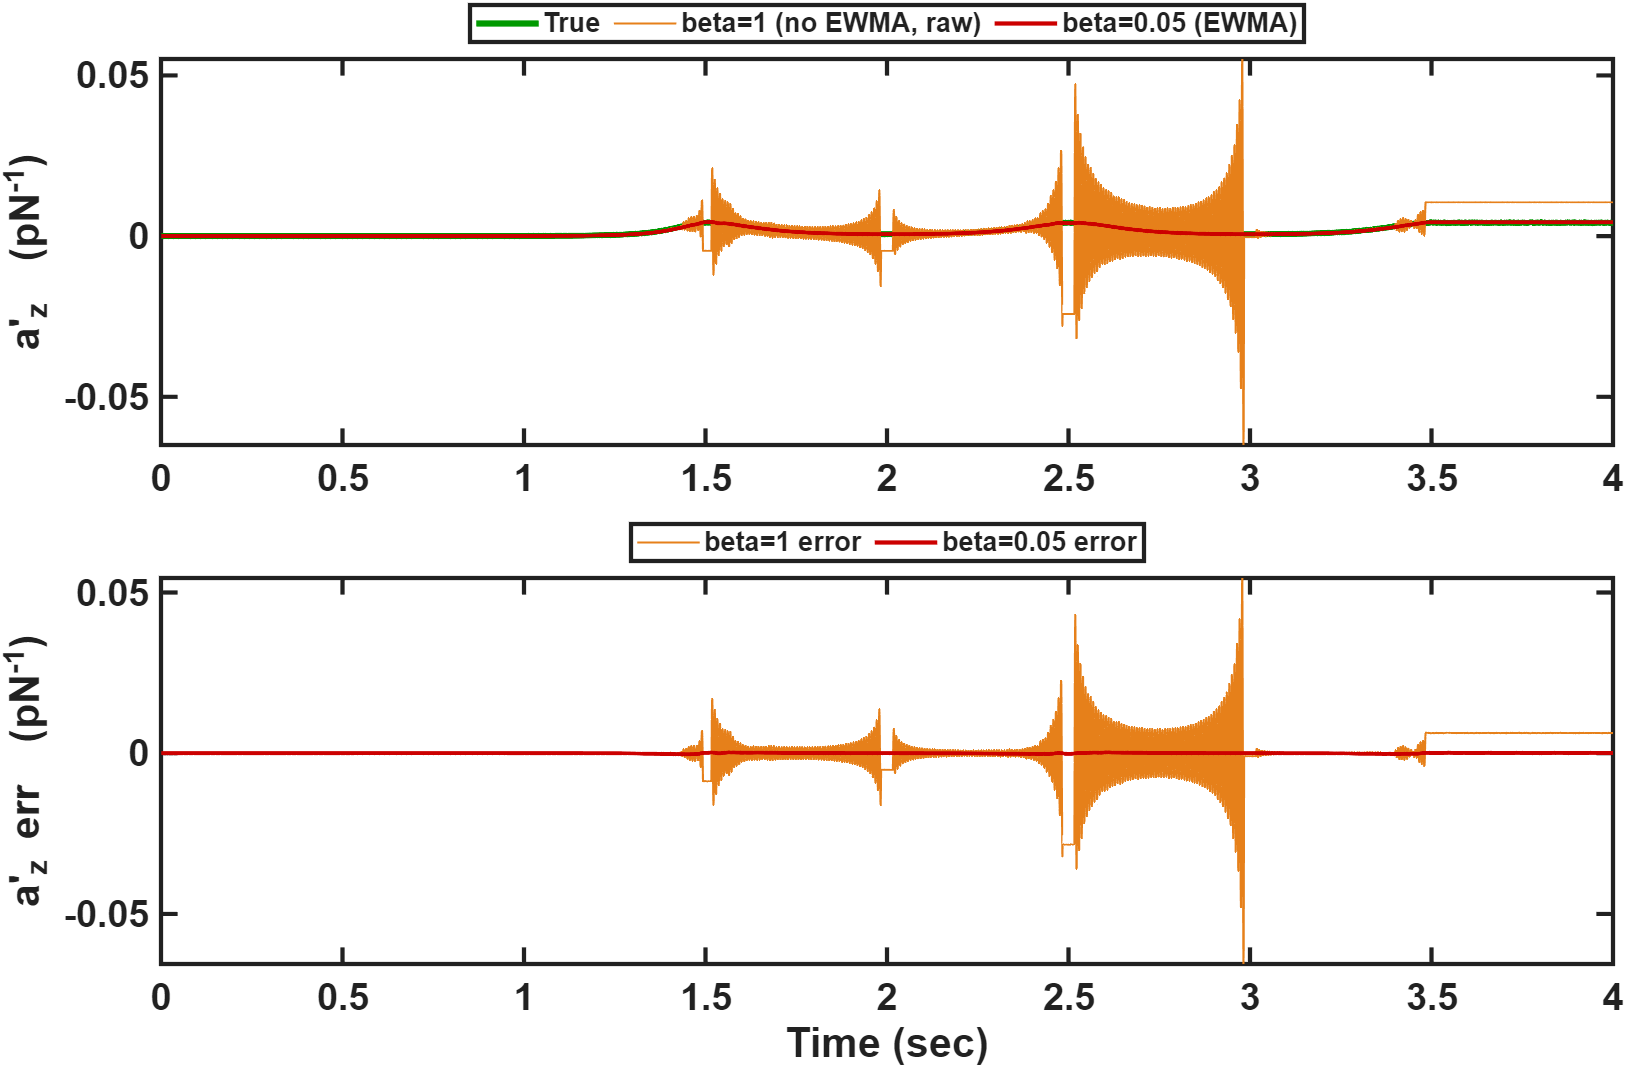
\includegraphics[width=0.85\textwidth]{figures/fig_aprime_ewma_compare_z.png}\\[0.4ex]
{\small\itshape Layer 1 --- self-differenced $a'_z$, raw ($\beta=1$) vs EWMA-smoothed ($\beta=0.05$): corr$_z$ $0.36\to0.997$. Smoothing alone does most of the work.}
\end{minipage}

\medskip
\noindent\begin{minipage}{\linewidth}\centering
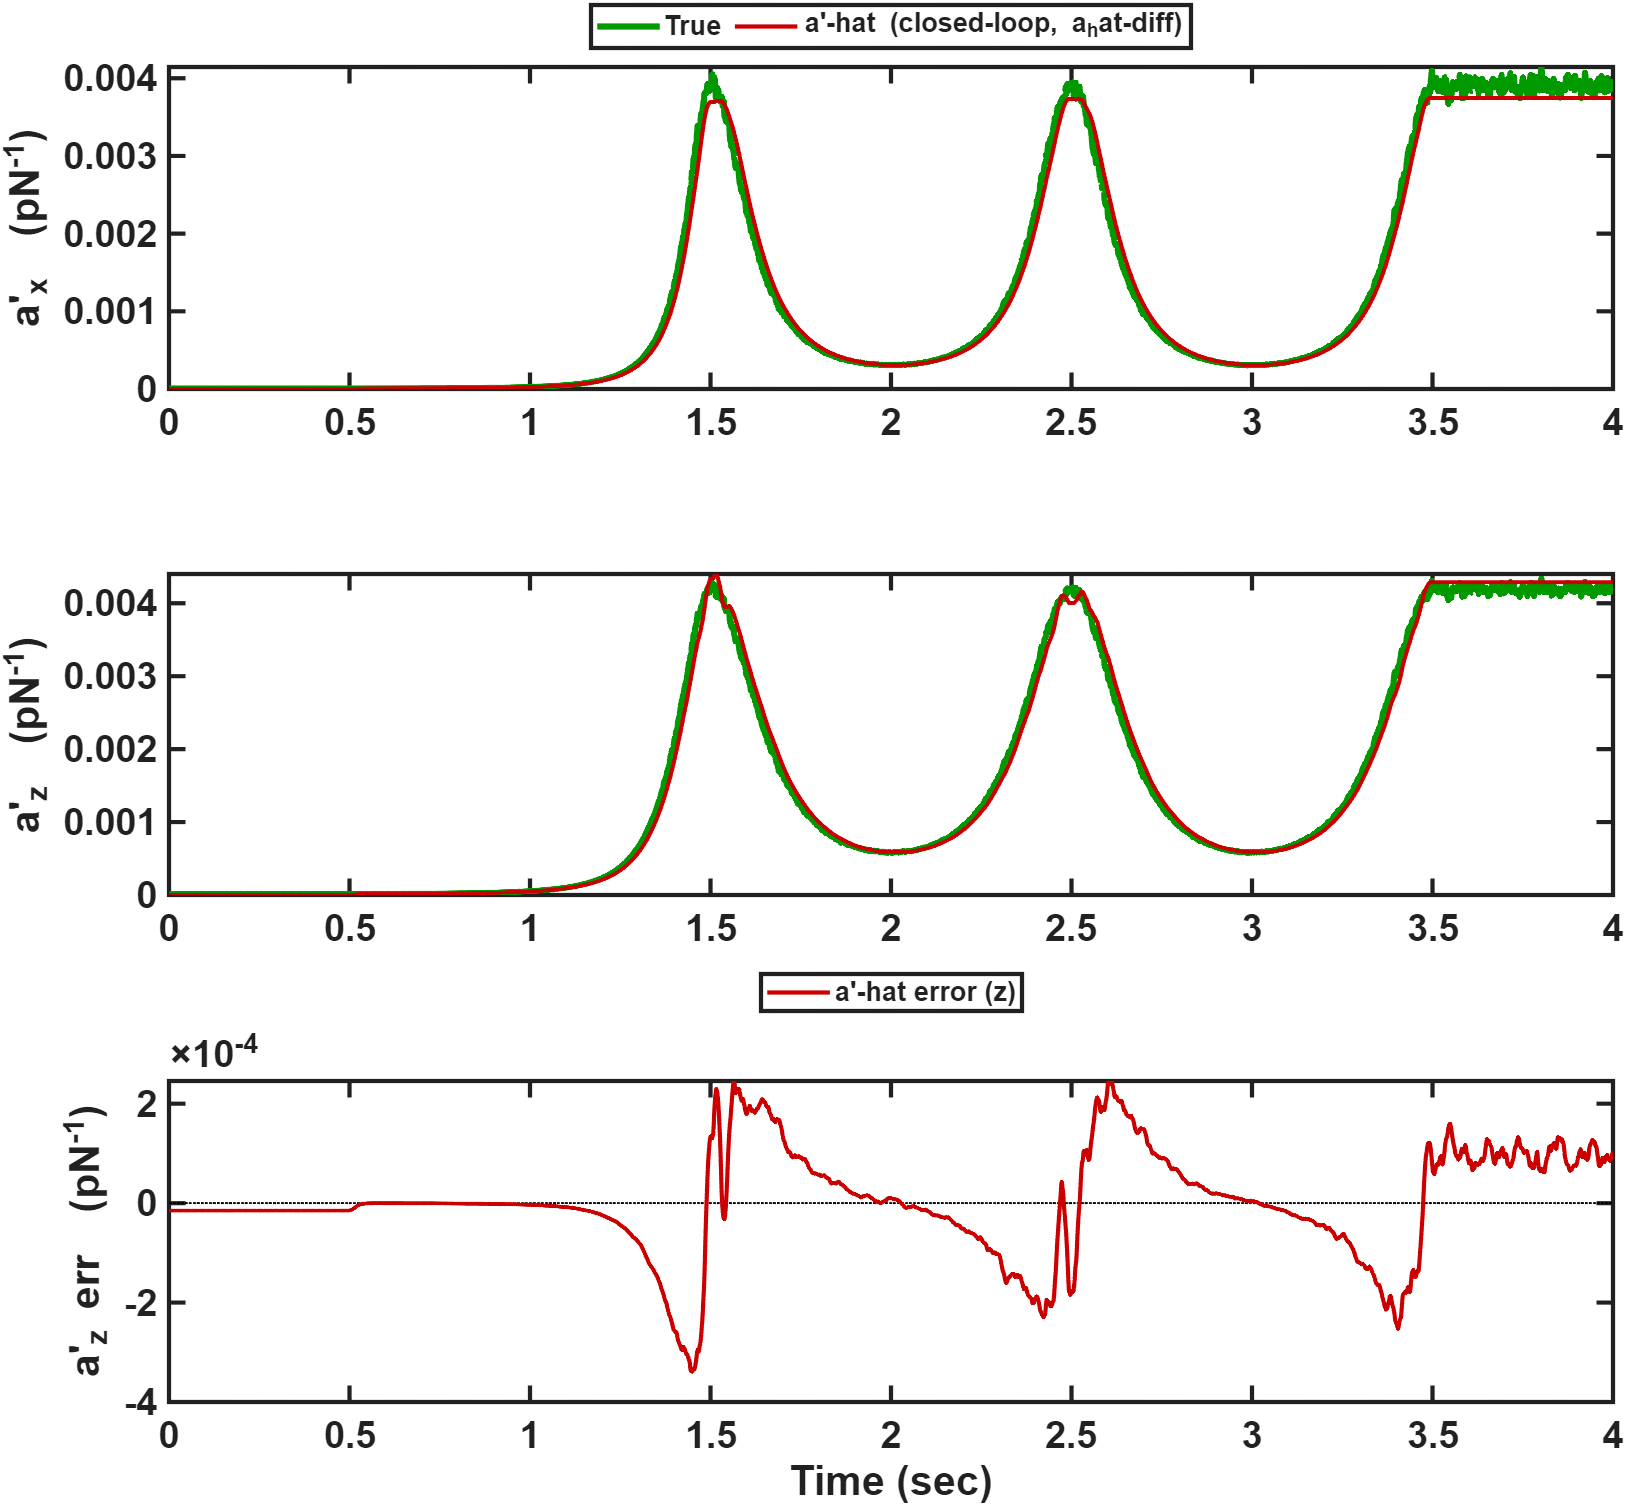
\includegraphics[width=0.85\textwidth]{figures/fig_aprime_ff_closedloop_z.png}\\[0.4ex]
{\small\itshape Layer 2 --- same smoothed estimate, full closed loop, $\hat a_{x_{det}}$ still known-wall: corr$=0.99$, but circular ($\hat a_x\approx a_{x_{det}}$, riding on the smoothing above).}
\end{minipage}

\medskip
\noindent\begin{minipage}{\linewidth}\centering
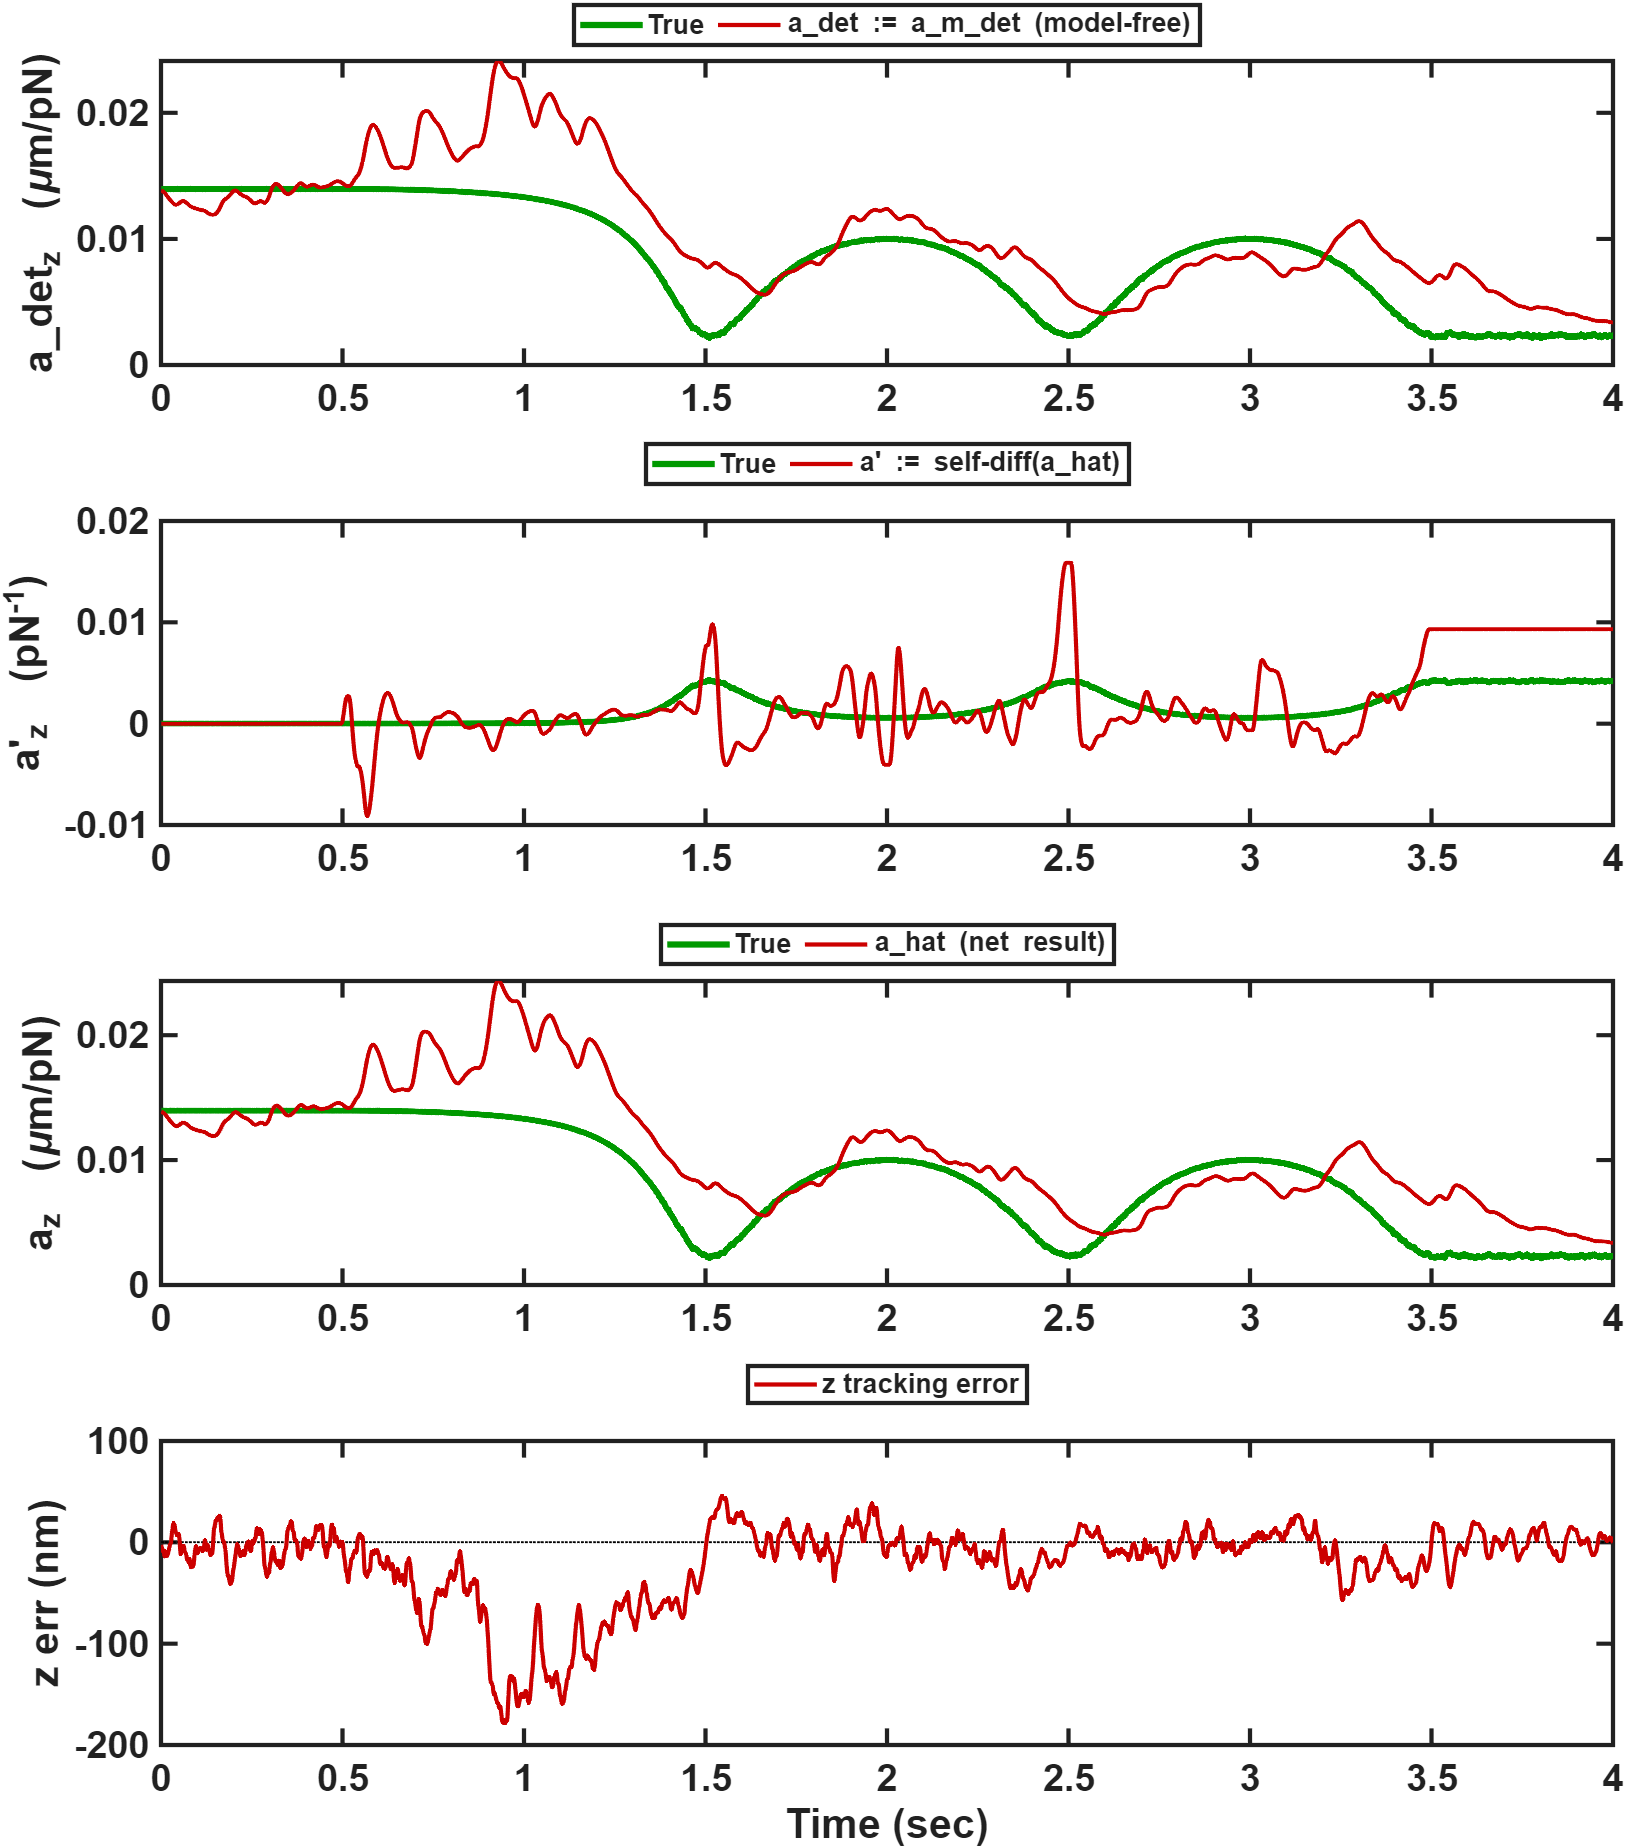
\includegraphics[width=0.9\textwidth]{figures/fig_nocheat_z.png}\\[0.4ex]
{\small\itshape Layer 3 --- both $\hat a_{x_{det}}$ and $\hat a'_x$ model-free, stable ($0/3$ diverge): $a_{x_{det}}$ corr$=0.70$; $a'_x$ corr$=0.27$ (weak link, honest number).}
\end{minipage}

\hd{Corrected error dynamics}
The estimator predict becomes $\hat a_x[k+1]=\lc\hat a_x[k]+(1-\lc)\hat a_{x_{det}}[k]+\hat a'_x[k]\Delta h_d[k]$. Subtracting from the true dynamics ($a_x[k+1]=\lc a_x[k]+(1-\lc)a_{x_{det}}[k]+\Delta a_x[k]+a'_x\varepsilon[k]$, boxed above):
\begin{empheq}[box=\fbox]{equation*}
e_{a_x}[k+1] = \lc\,e_{a_x}[k] \;+\; (1-\lc)\,e_{a_{x_{det}}}[k] \;+\; e_{a'_x}[k]\,\Delta h_d[k] \;+\; a'_x\,\varepsilon[k]
\end{empheq}
Two new noise terms appear (boxed); the original term $a'_x\varepsilon[k]$ is unchanged. $\mathbf F_e$ and $\mathbf H$ keep their original $4\times4$/$2\times4$ form --- $\hat a_{x_{det}}$ and $\hat a'_x$ enter as exogenous inputs, exactly like $a_{x_{det}}$ and $a'_x$ did; only $Q_{44}$, $R_{22}$ change.

\hd{Corrected $Q_{44}$, $R_{22}$}
The output equation's known correction $\sum_{i=1}^{d}\Delta a_x[k-i] = a_{x_{det}}[k]-a_{x_{det}}[k-d] \approx a'_x[k]\,\Delta H_d[k]$ ($\Delta H_d[k]:=h_d[k]-h_d[k-d]$, small-$d$ telescoping approx., already implicit in the parameter model) is now computed as $\hat a'_x[k]\,\Delta H_d[k]$, feeding the same $e_{a'_x}$ into the measurement side:
\begin{empheq}[box=\fbox]{align*}
Q_{44}^{\mathrm{new}}[k] &= \underbrace{(3-2\lc^2)\,a_x'^2\,\sigma^2_{\delta h}}_{q_4,\ \text{original}} \;+\; (1-\lc)^2\,\mathrm{Var}(e_{a_{x_{det}}})[k] \;+\; \Delta h_d[k]^2\,\mathrm{Var}(e_{a'_x})[k] \\
R_{22}^{\mathrm{new}}[k] &= \underbrace{R_{22}^{\mathrm{intrinsic}}+R_{22}^{\mathrm{delay}}}_{\text{original}} \;+\; \Delta H_d[k]^2\,\mathrm{Var}(e_{a'_x})[k]
\end{empheq}
\textbf{Assumption}: the three driving noises ($a'_x\varepsilon$, $e_{a_{x_{det}}}$, $e_{a'_x}$) are mutually independent -- revisit if not.

\hd{$\mathrm{Var}(e_{a_{x_{det}}})$ --- closed form}
$\hat a_{x_{det}}$ is a first-moment EWMA of $a_{xm}[k]=a_x[k-d]+n_a[k]$ ($n_a$: variance $=R_{22}$, the $a_{xm}$ measurement noise derived in the companion $a_{xm}$ documents). Standard EWMA group delay $\tau_\alpha=(1-\alpha)/\alpha$ samples, plus the EWMA noise-gain $\alpha/(2-\alpha)$ (same form as $K_{\mathrm{var}}$'s $g_E$ factor elsewhere in this line):
\begin{empheq}[box=\fbox]{equation*}
\mathrm{Var}(e_{a_{x_{det}}})[k] \;\approx\; \underbrace{\Big(\Delta a_x[k]\cdot\tfrac{1-\alpha}{\alpha}\Big)^{2}}_{\text{EWMA lag bias}} \;+\; \underbrace{\tfrac{\alpha}{2-\alpha}\,R_{22}[k]}_{\text{noise averaging}}
\end{empheq}
\textbf{Impl.}: $\alpha=$ \texttt{a\_det\_lp} (currently $0.005$, inherited from an unrelated, now-superseded role -- \emph{never} tuned as the AR(1) reversion target's own bandwidth). At $\alpha=0.005$, $\tau_\alpha\approx199$ samples; the lag term is suspected to dominate for a fast (1\,Hz) trajectory. A sweep of $\alpha$ trades the lag term against the noise term -- the same lag$\leftrightarrow$noise trade-off as the $Q_{55}$ $\kappa$-sweep in the companion \texttt{5state\_est\_aprime} line.

\hd{$\mathrm{Var}(e_{a'_x})$ --- self-referential, closed form under two stated approximations}
$\hat a'_x[k]$ is differenced from $\hat a_x$'s own history, so $e_{a'_x}[k]$ is a function of $e_{a_x}[k]-e_{a_x}[k-1]$ -- \emph{self-referential} with the very quantity $Q_{44}^{\mathrm{new}}$ is meant to bound (same structural family as the $a_{x_{det}}:=\hat a_x$ closed-loop instability, Exp.~03 in the companion status note, but here at the level of noise statistics rather than outright divergence). A closed form IS derivable, under two named approximations: \textbf{(A)} $\Delta h_d$ locally constant over the EWMA window; \textbf{(B)} $e_{a_x}$'s driving noise treated as white when computing $e_{a_x}$'s own autocorrelation (ignores that $e_{a_{x_{det}}}$, $e_{a'_x}$ are themselves EWMA outputs and hence colored -- the same order of simplification as the Q33 ``Path C'' treatment elsewhere in this project line).

\textit{Step 1 --- unroll the EWMA.} With $r[k]:=[\hat a_x[k]-\hat a_x[k-1]]/\Delta h_d[k-1]$ and $d[k]:=e_{a_x}[k]-e_{a_x}[k-1]$ (so $a'_x[k]-r[k]=d[k]/\Delta h_d[k-1]$, boxed earlier):
\[ \hat a'_x[k] = \beta\textstyle\sum_{j\ge0}(1-\beta)^j r[k-j] \;\;\Rightarrow\;\; e_{a'_x}[k] \approx \frac{\beta}{\Delta h_d[k-1]}\textstyle\sum_{j\ge0}(1-\beta)^j\,d[k-j] \]

\textit{Step 2 --- model $e_{a_x}$ as AR(1), pole $\lc$ (approximation B).} Standard AR(1) increment/autocorrelation identities (same form as $\mathrm{Var}(\Delta x_{ram})$ earlier):
\[ \mathrm{Var}(d) = 2(1-\lc)\,P_a, \qquad \rho_d(\tau) = -\tfrac{1-\lc}{2}\,\lc^{\tau-1} \;\;(\tau\ge1) \]

\textit{Step 3 --- EWMA variance transfer} (linear, no Isserlis needed -- $d$ itself, not $d^2$, is being averaged): the color sum telescopes exactly,
\[ 1+2\textstyle\sum_{\tau\ge1}\rho_d(\tau)\,s^\tau = \frac{\beta}{1-\lc(1-\beta)}, \qquad s:=1-\beta \]
\begin{empheq}[box=\fbox]{equation*}
\mathrm{Var}(e_{a'_x}) \;\approx\; \frac{2\beta^2(1-\lc)}{(2-\beta)\big[1-\lc(1-\beta)\big]}\cdot\frac{P_a}{\Delta h_d[k-1]^2}
\end{empheq}

\textit{Step 4 --- self-consistency} (substitute into $Q_{44}^{\mathrm{new}}$, $\Delta h_d[k]\approx\Delta h_d[k-1]$, impose $P_a=Q_{44}^{\mathrm{new}}/(1-\lc^2)$):
\begin{empheq}[box=\fbox]{equation*}
P_a = \frac{q_4+(1-\lc)^2\mathrm{Var}(e_{a_{x_{det}}})}{(1-\lc)\Big[(1+\lc)-\dfrac{2\beta^2}{(2-\beta)[1-\lc(1-\beta)]}\Big]}
\end{empheq}
$\mathrm{Var}(e_{a'_x})$ then follows by plugging this $P_a$ back into the Step 3 box.

\textbf{Stability condition}: $P_a\ge0$ requires the bracket $>0$, i.e.\ $(1+\lc) > \dfrac{2\beta^2}{(2-\beta)[1-\lc(1-\beta)]}$ -- a closed-form bound on how little smoothing ($\beta$) the self-differenced $a'$ can tolerate before the self-consistent variance has no valid solution. \textbf{Check} ($\lc=0.7$): $\beta=0.05\Rightarrow$ bracket$\,\approx1.69>0$ (stable, matches the verified test config); $\beta=1$ (raw, no smoothing) $\Rightarrow$ bracket $=-0.3<0$ -- no valid $P_a$, consistent with the empirically observed instability of un-smoothed self-differencing.

\textbf{Caveat}: this is a closed form \emph{under approximations (A) and (B)} -- not an exact result. (B) in particular ignores that $e_{a_{x_{det}}}$ and $e_{a'_x}$ are themselves colored (EWMA outputs), so the true $\rho_d(\tau)$ has additional structure beyond the pure-AR(1) form used here; treat the stability boundary as indicative, not exact, and prefer the closed-loop empirical test (Exp.\ nocheat above) as the final check.

\newpage
\hd{FALSIFICATION --- $e_{a_{x_{det}}}$ is NOT exogenous in closed loop}
The corrected $Q_{44}^{\mathrm{new}}$ above was implemented and tested on the failing scenario: \textbf{no effect} (bias $+11.9\%\to+12.2\%$). Loop-cut interventions on the same scenario: (i) control law fed the \emph{true} gain (estimator untouched) $\Rightarrow$ fully stable, open-loop anchor bias only $1.6$--$3.7\%$; (ii) $y_2$ KF channel permanently off $\Rightarrow$ blow-up \emph{bit-identical} to the closed-loop run. Hence the destabilizing coupling enters through the \emph{real tracking error} into the predict-side anchor ($\hat a_{x_{det}}\to$ predict, fixed weight $1-\lc$, no Kalman damping) --- a path that no $Q$/$R$ re-weighting can see. The exogeneity assumption behind $Q_{44}^{\mathrm{new}}$ is falsified; the sections below replace it with the explicit coupling.

\hd{The $g$-mismatch closed loop}
Let $g[k] := a_x[k]/\hat a_x[k]$ (gain mismatch; control uses $\hat a_x$). Re-deriving the closed loop from the implementable control effort (boxed near the top of this document) \emph{without} assuming $\hat a_x = a_x$, quasi-static $g$ over the $d{+}1$ window:
\begin{empheq}[box=\fbox]{equation*}
\delta x[k+1] = \lc\,\delta x[k] \;+\; (1-g)(1-\lc)\,\delta x[k-d] \;+\; (1-g)\,D[k] \;-\; \varepsilon_g[k]
\end{empheq}
\[
D[k] := x_d[k+1] - \lc\,x_d[k] - (1-\lc)\,x_d[k-d]
\]
\[
\varepsilon_g[k] := a_x f_T[k] + (1-\lc)\textstyle\sum_{i=1}^{d} a_x f_T[k-i] - g(1-\lc)\,n_x[k]
\]
$D[k]$ is a \emph{known} trajectory functional ($=0$ during holds). Self-check $g=1$: reduces to $\lc\,\delta x - \varepsilon$ with $\mathrm{Var}(\varepsilon) = 4k_BT a_x(1+(1-\lc)^2 d) + (1-\lc)^2\sigma^2_{n_x}$ --- identical to $Q_{33}$ at $f_d=0$. \textbf{Validation} (fixed-$g$ probe, noise-free osc): corr $=1.0000$, amplitude ratio $1.000$, rel.\ RMS $\le 0.3\%$ at $g=0.5$ and $g=2$.

\textbf{$\delta p_{md}$ is the hidden $g$ channel}: the deterministic response is, quasi-statically,
\[
\delta x_{det}[k] \;\approx\; \frac{(1-g)\,D[k]}{g\,(1-\lc)}
\]
(DC gain of the loop above), and this is precisely the content of the LP output $\delta p_{md}$ --- a \emph{signed, first-moment} measurement of $g$ that the estimator chain currently discards.

\hd{Variance map under mismatch}
Augmenting $[\delta x[k], \delta x[k-1], \delta x[k-2], w[k-1], w[k-2], b[k-1]]$ ($w := a_x f_T$, $b$ the $a_{pd}$-LP state) and solving the discrete Lyapunov equation gives the HP-residual variance as a $g$-family:
\begin{empheq}[box=\fbox]{equation*}
\mathrm{Var}(\delta x_r)(g) \;=\; c_w(g)\cdot 4k_BT\,a_x \;+\; c_n(g)\cdot \sigma^2_{n_x}
\end{empheq}
with the consistency check $c_w(1)\cdot 4k_BT a_x + c_n(1)\,\sigma^2_{n_x} \equiv C_{\mathrm{dpmr}}\,4k_BT a_x + C_n \sigma^2_{n_x}$.
\textbf{Validation} (hold at $\bar h = 2.22$, five fixed $g$): predicted vs measured within $0.1$--$0.5\%$; the $g=1$ cross-check reproduces the $C_{\mathrm{dpmr}}$ formula to ratio $1.0000$. The confound in numbers: $a_{xm}/a_x = 1.22$ at $g=0.6$, $0.93$ at $g=1.67$ --- overestimating $\hat a_x$ inflates $a_{xm}$, which (fed back as the anchor) pushes $\hat a_x$ further up: positive feedback with loop strength $\propto \alpha$. At hold the DC loop gain is $\approx 0.31 < 1$ (statically stable), so the cliff requires trajectory motion plus noise.

\hd{Mechanism closure --- bias and the $\alpha$ cliff}
A scalar surrogate built from ONLY the two boxed results above (no EKF, no $y_1/y_2$, no 3-axis physics):
\begin{itemize}[leftmargin=*,topsep=0pt,itemsep=0pt]
\item \emph{Mean path}: reproduces the closed-loop bias ($26.1\%/10.6\%$ predicted vs $25.5\%/11.9\%$ measured at $\alpha=0.002/0.005$) but stays stable to $\alpha=0.05$ $\Rightarrow$ the bias is a mean-path (lag $+$ loop-equilibrium) effect, the cliff is not.
\item \emph{With correlated noise sampling}: cliff appears at the measured location ($0.007\to0/5$, $0.008\to1/5$, $0.010\to3/5$, $0.020\to5/5$; real simulator: $0.005$ stable, $0.008$ blown) $\Rightarrow$ the cliff is noise-triggered escape ($\chi^2$ fluctuation of $\hat\sigma^2_{\delta x_r}$, rel.\ std $\sim46\%$, amplified through the nonlinear $g$-loop).
\item \emph{Counter-side (oracle)}: restoring the missing $g$-dependence inside the fully closed loop (true $g$, correction below) collapses the bias to $+4.1\%$ and removes the cliff ($0.008, 0.010 \to 0/3$).
\end{itemize}

\hd{Deployable $\hat g$ estimator from $\delta p_{md}$ (model-free)}
Apply the SAME LP and $d$-step delay to the known regressor: $\bar D[k] := \mathrm{LP}_{a_{pd}}(D[k-d])$, so that lags match:
\[
\mathrm{E}\{\delta p_{md}[k]\} \;\approx\; \frac{1-g}{g\,(1-\lc)}\;\bar D[k]
\]
The pointwise ratio $u = (1-\lc)\,\delta p_{md}/\bar D$ FAILS in practice (per-sample SNR $<1$; ratio rectification --- tested: bias $+52.9\%$, worse than uncorrected). The \textbf{regression form} is required --- excitation-weighted, and unbiased because $\bar D$ is deterministic ($\mathrm{E}\{\bar D\cdot\text{noise}\}=0$):
\begin{empheq}[box=\fbox]{equation*}
S_{xy} = \mathrm{EWMA}_{\beta_g}(\bar D\,\delta p_{md}),\quad
S_{xx} = \mathrm{EWMA}_{\beta_g}(\bar D^2),\quad
u = (1-\lc)\frac{S_{xy}}{S_{xx}},\quad
\hat g = \mathrm{clamp}\Big(\frac{1}{1+u},\,[0.5,\,2]\Big)
\end{empheq}
$\hat g$ held at its previous value while $S_{xx} \le \gamma_D^2$ (insufficient excitation, e.g.\ holds). Test values: $\beta_g = 0.05$, $\gamma_D = 2\times10^{-3}\,\mu$m. (Slower $\beta_g=0.02$ was tested and rejected: estimator lag destabilizes at higher $\alpha$.)

\hd{Corrected inversion and anchor (deployable)}
Run the deterministic-leak predictor with $\hat g$ (same recursion as the boxed $g$-mismatch loop, driven by the known $D[k]$), pass it through the same LP/HP as the measurement chain, and restore the $g$-dependence of the inversion:
\[
\delta x_{det}[k+1] = \lc\,\delta x_{det}[k] + (1-\hat g)(1-\lc)\,\delta x_{det}[k-d] + (1-\hat g)\,D[k]
\]
\[
\hat\sigma^2_{det} = \mathrm{EWMA}_{a_{cov}}\big(\mathrm{HP}_{a_{pd}}(\delta x_{det}[k-d])^2\big)
\]
\begin{empheq}[box=\fbox]{equation*}
a_{xm}^{corr}[k] = \frac{\hat\sigma^2_{\delta x_r}[k] - \hat\sigma^2_{det}[k] - c_n(\hat g)\,\sigma^2_{n_x}}{c_w(\hat g)\cdot 4k_BT},
\qquad
\hat a_{x_{det}}[k+1] = (1-\alpha)\,\hat a_{x_{det}}[k] + \alpha\,a_{xm}^{corr}[k]
\end{empheq}
Only the anchor consumes $a_{xm}^{corr}$; the $y_2$ channel keeps the raw $a_{xm}$ (proven irrelevant by the loop-cut). $c_w(\cdot), c_n(\cdot)$ from a lookup over $\log g$ built offline (depends only on $\lc, a_{pd}$ --- no $c(\bar h)$).

\hd{Complete controller (unknown $c(\bar h)$, wall position known)}
Everything else in this document is unchanged. The full per-axis loop:
\begin{enumerate}[leftmargin=*,topsep=0pt,itemsep=0pt]
\item Control effort: boxed implementable form (top of document), $\hat a_x$ from the EKF.
\item EKF: 4-state AR(1), $F_e$/$H$/$Q_{33}$/$Q_{44}$/$R$ unchanged; predict $\hat a_x[k+1] = \lc\hat a_x[k] + (1-\lc)\hat a_{x_{det}}[k] + \hat a'_x[k]\Delta h_d[k]$.
\item $\hat a'_x$: gated+EWMA self-difference of $\hat a_x$ (boxed earlier; zero-cost, ablation-verified).
\item $\hat g$: regression estimator from $\delta p_{md}$ (boxed above).
\item $a_{xm}^{corr}$, $\hat a_{x_{det}}$: corrected inversion and anchor (boxed above).
\end{enumerate}
Residual known-model dependencies, declared out of scope for this line: $K_h$ inside the $Q_{44}$/$R_{22}$ random-gain floor, and the wall-aware $\hat a_x[0]$ seed.

\hd{End-to-end validation (osc\_1hz, near wall, z-axis)}
\begin{center}
\begin{tabular}{llrrr}
\toprule
variant & $\alpha$ & blown & track$_z$ (nm) & bias$_z$ (\%) \\
\midrule
known wall (baseline)        & --    & 0/3 & 24.1 & 0.0 \\
model-free, uncorrected      & 0.005 & 0/3 & 34.9 & $+12.2$ \\
model-free, uncorrected      & 0.008 & --  & \multicolumn{2}{c}{blown ($>1500$ nm)} \\
oracle $g$ (upper bound)     & 0.005 & 0/3 & 27.9 & $+4.1$ \\
oracle $g$ (upper bound)     & 0.010 & 0/3 & 28.8 & $+1.6$ \\
\textbf{deployable} ($\hat g$ from $\delta p_{md}$) & \textbf{0.005} & \textbf{0/5} & \textbf{30.5} & $\bm{+3.2}$ \\
deployable                   & 0.008 & 1/5 & 34.0 & $+0.4$ \\
deployable                   & 0.010 & 1/5 & 47.6 & $+0.1$ \\
deployable                   & 0.020 & 5/5 & \multicolumn{2}{c}{blown} \\
\bottomrule
\end{tabular}
\end{center}
Operating point: $\alpha = 0.005$ (0/5 seeds, all axes $28$--$31$ nm, gain bias $\le 5.5\%$ all axes), safety margin to the cliff $\approx 1.6\times$. The deployable controller recovers most of the oracle's gain: bias $+12.2\%\to+3.2\%$ at the cost of $\sim6$ nm tracking vs the known-wall baseline.

\end{document}
